\newpage

\section{Smart Pointer}

A smart pointer is a C++ class that mimics a regular pointer in syntax
and some semantics, but it does more.
\begin{verbatim}
template <class T>
class SmartPtr{
public:
  explicit SmartPtr(T* pointee) : pointee_(pointee);
  SmartPtr& operator=(const SmartPtr& other);
  ~SmartPtr();
  T& operator*() const{
    ...
    return *pointee_;
  }
  T* operator->() const{
    ...
    return pointee_;
  }
private:
  T* pointee_;
  ...
};
\end{verbatim}

\texttt{SmartPtr<T>} aggregates a pointer to \texttt{T} in its member
variable \texttt{pointee\_}. That's what most smart pointers do. In
some cases, a smart pointer might aggregate some handles to data and
compute the pointer on the fly.

\subsection{The Deal with Smart Pointer}

\textbf{Smart pointers have value semantics, whereas some simple
pointers do not, which means you can \emph{copy} and \emph{assign
  to}}.

\begin{verbatim}
Widget* p = new Widget;
\end{verbatim}
the variable p not only points to, but also owns, the memory allocated
for the \texttt{Widget} object, because later you must issue delete p
to ensure that the Widget object is destroyed and its memory is 
released. Furthermore, when you copy p into another variable, all you
get is two raw pointers pointing to the same object, and you have to
track them even more carefully because double deletions are even more
catastrophic than no deletion.

Smart pointers can be of great help in this area. Most smart pointers
offer \textbf{ownership management} in addition to pointer-like
behavior. Smart pointers can figure out how ownership evolves, and their
destructors can release the memory according to a well-defined
strategy:
\begin{itemize}
\item Some
smart pointers transfer ownership automatically: after you copy a
smart pointer to an object, the source smart pointer becomes
null. This is the behavior implemented by the standard-provided
\texttt{std::auto\_ptr}.
\item Other smart pointers implement reference counting: They track
  the total count of smart pointers that point to the same object, and
  when this count goes down to zero, they delete the pointed-to object.
\end{itemize}

However, you will find that adding seemingly worthwhile features might
expose the clients to costly risks.

\subsection{Storage (Policy) of Smart Pointers}

There are two generalizations of smart pointers:

Firstly, When you apply \texttt{operator->} to a type that's not a
built-in pointer, the compiler does an interesting thing. After
looking up and applying the user-defined \texttt{operator->} to that
type, it applies \texttt{operator->} again to the result. So \textbf{a
smart pointer's \texttt{operator->} does not have to return a
pointer.}

Secondly,  in rare cases, smart pointers could drop the pointer
syntax. An object that does not define \texttt{operator->} and
\texttt{operator*} violates the definition of a smart pointer, but
there are objects that \textbf{do deserve smart pointer–like
treatment}, although they are not, strictly speaking, smart pointers.

For example, in real-world APIs and applications, many operating
systems foster handles as accessors to certain internal resources.
Handles are intentionally obfuscated pointers, one of their purposes
is to prevent their users from manipulating critical operating system
resources directly.  Most of the time, handles are integral values
that are indices in a hidden table of pointers. The table provides the
additional level of indirection that protects the inner system from
the application programmers. Although they don't provide an
\texttt{operator->}, handles resemble pointers in semantics and in the
way they are managed.

To generalize the type universe of smart pointers, we distinguish
three potentially distinct types in a smart pointer:
\begin{enumerate}
\item \textbf{The storage type}. This is the type of
  \texttt{pointee\_}. By "default"—in regular smart pointers—it is a
  raw pointer. 
\item \textbf{The pointer type}. This is the type returned by
  \texttt{operator->}. It can be different from the storage type if
  you want to return a proxy object instead of just a pointer. (You
  will find an example of using proxy objects later in this chapter.)
\item \textbf{The reference type}. This is the type returned by
  \texttt{operator*}
\end{enumerate}
There three types are called Storage policy.

\subsection{Smart Pointer Member Functions}

Many existing smart pointer implementations allow operations through
member functions, such as \texttt{Get} for accessing the
\texttt{pointee} object, \texttt{Set} for changing it, and
\texttt{Release} for taking over ownership.

However, the interaction between member function calls for the smart
pointer for the pointed-to object can be extremely confusing.
\begin{verbatim}
SmartPtr<Printer> spRes = ...;
spRes->Acquire(); // acquire the printer
spRes->Release(); // release the printer
spRes.Release(); // release the pointer to the printer
\end{verbatim}

Both \texttt{sp.Release()} and \texttt{sp->Release()} compile
flag-free but do very different things. The cure is simple: \textbf{A smart
pointer should not use member functions.} \texttt{SmartPtr} use only 
nonmember functions. These functions become friends of the smart
pointer class. 

The only functions that necessarily remain members of
\texttt{SmartPtr} are the constructors, the destructor,
\texttt{operator=}, \texttt{operator->}, and unary
\texttt{operator*}. All other operations of SmartPtr are provided
through named nonmember functions.
\begin{verbatim}
template <class T> T* GetImpl(SmartPtr<T>& sp);
template <class T> T*& GetImplRef(SmartPtr<T>& sp);
template <class T> void Reset(SmartPtr<T>& sp, T* source);
template <class T> void Release(SmartPtr<T>& sp, T*& destination);
\end{verbatim}

\begin{itemize}
\item \texttt{GetImpl} returns the pointer object stored by \texttt{SmartPtr}.
\item \texttt{GetImplRef} returns a reference to the pointer object stored by
  \texttt{SmartPtr}. GetImplRef allows you to change the underlying pointer, so
  it requires extreme care in use.
\item \texttt{Reset} resets the underlying pointer to another value,
  releasing the previous one. 
\item \texttt{Release} releases ownership of the smart pointer, giving
  its user the responsibility of managing the pointee object's lifetime.
\end{itemize}

\subsection{Ownership (Policy) Strategies}

A smart pointer is a first-class value that takes care of deleting the
pointed-to object under the covers.  For implementing self-ownership,
smart pointers must carefully track the pointee object, especially
during copying, assignment, and destruction.

\subsubsection{Deep Copy}
The simplest strategy applicable is to copy the pointee object
whenever you copy the smart pointer. If you ensure this, \textbf{there is only
  one smart pointer for each pointee object. } But why would you make
the effort of using a smart pointer, when simple pass by value of the
pointee object works just as well?

The answer is \textbf{support for polymorphism.} Smart pointers are
vehicles for transporting polymorphic objects safely. When you
copy the smart pointer, you want to copy its polymorphic behavior,
too.

However,  the following naive implementation of the
copy constructor is wrong:
\begin{verbatim}
template <class T>
class SmartPtr{
public:
  SmartPtr(const SmartPtr& other): pointee_(new T(*other.pointee_)){}
};
\end{verbatim}
The copy constructor above copies only the \texttt{Widget} part of
the \texttt{ExtendedWidget} object. This phenomenon is known as
\textbf{slicing}.

Chapter 8 discusses cloning in depth. As shown there, the classic way
of obtaining a polymorphic clone for a hierarchy is to define a
virtual \texttt{Clone} function and implement it as follows:
\begin{verbatim}
class AbstractBase{
  virtual Base* Clone() = 0;
};
class Concrete : public AbstractBase{
  virtual Base* Clone(){ return new Concrete(*this); }
};
\end{verbatim}

A generic smart pointer cannot count on knowing the exact name of the
cloning member function—maybe  it's \texttt{clone}, or maybe
\texttt{MakeCopy}. Therefore, the most flexible approach is to
parameterize \texttt{SmartPtr} with a policy that addresses cloning.

\subsubsection{Copy on Write}
Copy on write is an optimization technique that avoids unnecessary
object copying. The idea that underlies COW is to \textbf{clone the pointee
object at the first attempt of modification; until then, several
pointers can share the same object.}

Smart pointers, however, are not the best place to implement COW,
because smart pointers cannot differentiate between calls to const and
non-const member functions of the pointee object. (\emph{pointer to
  non-const object can also call const member function}).

\subsubsection{Reference Counting}

Reference counting tracks the number of smart pointers that point to
the same object. When that number goes to zero, the pointee object is
deleted. This strategy works very well if you don't break certain
rules—\textbf{you should not keep dumb pointers and smart
  pointers to the same object.}

There are three structures:
\begin{itemize}
\item Each smart pointer holds \textbf{a pointer to the
reference counter}  in addition to the pointer to the object
itself. This usually \textbf{doubles the size of the smart pointer},
which may or may not be an acceptable amount of overhead, depending on
your needs and constraints.

There is another, subtler overhead issue. Reference-counted smart
pointers must store the reference counter on the free
store. \textbf{The problem is that in many implementations, the
  default C++ free store allocator is remarkably slow and wasteful of
  space when it comes to allocating small objects.}
\item The relative size overhead can be partially mitigated by holding
  the pointer and the reference count together, the structure  in the
  following figure reduces
  the size of the smart pointer to that of a pointer, but at the
  expense of access speed.
  \begin{figure}[H]
    \centering
    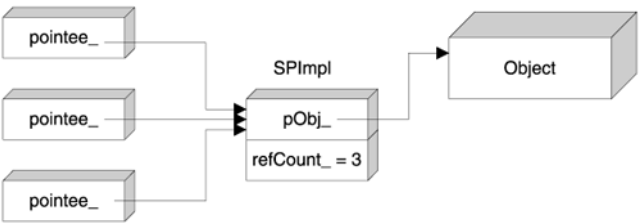
\includegraphics[width=0.7\textwidth]{fig/refCounter2.png}
  \end{figure}
\item The most efficient solution is to hold the reference counter in
  the pointee object itself, as shown in the following figure.
   \begin{figure}[H]
    \centering
    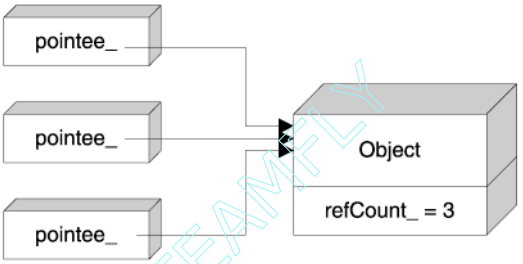
\includegraphics[width=0.7\textwidth]{fig/refCounter3.png}
  \end{figure}
  
  However, you must design up front or modify the pointee class to
  support reference counting. For implementing nonintrusive reference
  counting, the small-object allocator presented in Chapter 4 can help
  a great deal. 
\end{itemize}

\subsubsection{Reference Linking}

\begin{figure}[H]
    \centering
    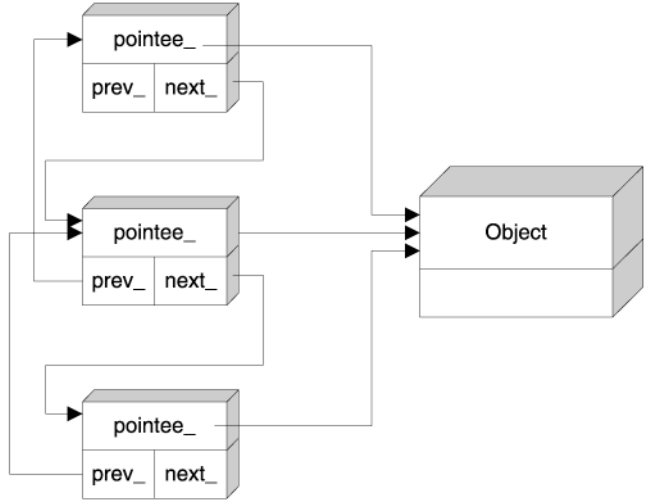
\includegraphics[width=0.7\textwidth]{fig/refLinking.png}
 \end{figure}

When you create a new \texttt{SmartPtr} from an existing
\texttt{SmartPtr}, the new object is appended to the list;
\texttt{SmartPtr}'s destructor takes care of removing the destroyed
object from the list. 

You cannot use a singly linked list or vector because removals from
such a list take linear time.

The advantage of reference linking over reference counting is that the
former does not use extra free store, which makes it more reliable:
Creating a reference-linked smart pointer cannot fail.

The disadvantage is that reference linking needs more memory for its
bookkeeping and reference counting should be a bit speedier. You
should use reference linking only when the free store is scarce.

There is  a significant disadvantage of reference management—be it
counting or linking—is \textbf{a victim of the resource leak known as
  cyclic reference}.  Imagine an object \texttt{A} holds a smart
pointer to an object \texttt{B}. Also, object \texttt{B} holds a smart
pointer to \texttt{A}. The reference management strategy cannot detect
such cyclic references, and the two objects remain allocated forever.

\subsubsection{Destructive Copy}

Destructive copy does exactly what you think it does: During copying,
it destroys the object being copied. Smart pointers may use
destructive copy to ensure that at any time there is only one smart
pointer pointing to a given object.
\begin{verbatim}
template <class T>
class SmartPtr{
public:
  SmartPtr(SmartPtr& src){
    pointee_ = src.pointee_;
    src.pointee_ = 0;
  }
  SmartPtr& operator=(SmartPtr& src){
    if (this != &src){
      delete pointee_;
      pointee_ = src.pointee_;
      src.pointee_ = 0;
    }
    return *this;
  }
};
\end{verbatim}

C++ etiquette calls for the right-hand side of the copy constructor
and the assignment operator to be a reference to a \texttt{const}
object. Classes that foster destructive copy break this convention for
obvious reasons.

Because they do not support value semantics, smart pointers with
destructive copy cannot be stored in containers and in general must be
handled with almost as much care as raw pointers.

On the bright side, smart pointers with destructive copy have
significant advantages:
\begin{itemize}
\item \textbf{They incur almost no overhead. }
\item \textbf{They are good at enforcing ownership transfer
    semantics.} In this 
  case, you use the "maelstrom effect" described earlier to your
  advantage: You make it clear that your function takes over the
  passed-in pointer.
\item \textbf{They are good as return values from functions.} If the smart
  pointer implementation uses a certain trick, you can return smart
  pointers with destructive copy from functions. This way, you can be
  sure that the pointee object gets destroyed if the caller doesn't
  use the return value.
\item They are excellent as stack variables in functions that have
  multiple return paths. You don't have to remember to delete the
  pointee object manually—the smart pointer takes care of this for
  you. 
\end{itemize}
The destructive copy strategy is used by the standard-provided
\texttt{std::auto\_ptr}.

\subsection{Implicit Conversion to Raw Pointer Types}

\begin{verbatim}
template <class T>
class SmartPtr{
public:
  operator T*() // user-defined conversion to T*{
    return pointee_;
  }
  ...
};
\end{verbatim}

However, they might become dangerous especially
when they expose handles to internal data, which is precisely the case
with the operator T* in the previous code. Passing the raw pointer
around defeats the inner workings of the smart pointer. Once 
unleashed from the confines of its wrapper, the raw pointer can easily
become a threat to program sanity again, just as it was before smart
pointers were introduced.

Another danger is that user-defined conversions pop up unexpectedly,
even when you don't need them.
\begin{verbatim}
SmartPtr<Something> sp;
// However, it goes undetected at compile time
delete sp;
\end{verbatim}

There are quite a few ways to prevent the delete call from compiling.
\begin{verbatim}
template <class T>
class SmartPtr{
public:
  operator T*(){ return pointee_; }
  operator void*(){ return pointee_; }
};
\end{verbatim}
A call to delete against such a smart pointer object is ambiguous. But
don't forget that disabling the delete operator was only a part of the
issue.

However, forbidding implicit conversion does not necessarily eliminate
all access to the raw pointer. Therefore, all smart pointers do
provide explicit access to their wrapped pointer via a call to a
function: 
\begin{verbatim}
void Fun(Something* p);
SmartPtr<Something> sp;
Fun(GetImpl(sp));
\end{verbatim}

\texttt{SmartPtr} provides this implicit conversion as a choice. The
default is on the safe side—no implicit conversions. Explicit access
is always available through the GetImpl function.

\subsection{Equality and Inequality}

Sometimes we expect the following tests to compile and run
as they do for a raw pointer:
\begin{verbatim}
SmartPtr<Something> sp1, sp2;
Something* p;
if (sp1) // Test 1: direct test for non-null pointer
if (!sp1) // Test 2: direct test for null pointer
if (sp1 == 0) // Test 3: explicit test for null pointer
if (sp1 == sp2) // Test 4: comparison of two smart pointers
if (sp1 == p) // Test 5: comparison with a raw pointer
\end{verbatim}

There is an unfortunate interference between the solution to the
previous issue (preventing delete from compiling) and a possible
solution to this issue. With one user-defined conversion to the
pointee type, you can accidentally call the \texttt{delete} operator against
the smart pointer. With two user-defined conversions 
(intentional ambiguity), you detect wrongful delete calls.

An additional user-defined conversion to \texttt{bool} helps, but you
allow \texttt{SmartPtr} to act as a \texttt{bool} in many more
situations than you actually wanted.

A true, complete, rock-solid solution to this dilemma is to go all the
way and overload each and every operator separately.
\begin{verbatim}
template <class T>
class SmartPtr{
public:
  bool operator!() const{ return pointee_ == 0; }
  inline friend bool operator==(const SmartPtr& lhs,const T* rhs){
    return lhs.pointee_ == rhs; 
  }
  inline friend bool operator==(const T* lhs,const SmartPtr& rhs){
    return lhs == rhs.pointee_; 
  }
  inline friend bool operator!=(const SmartPtr& lhs,const T* rhs){ 
    return lhs.pointee_ != rhs; 
  }
  inline friend bool operator!=(const T* lhs,const SmartPtr& rhs){
    return lhs != rhs.pointee_; 
  }
};
\end{verbatim}

We still haven't solved the problem completely. If you provide an
automatic conversion to the pointee type, there still is the risk of
ambiguities.
\begin{verbatim}
SmartPtr<Base> sp;
Derived* p;
if (sp == p) {}
\end{verbatim}

We can add templated versions of them:
\begin{verbatim}
template <class T>
class SmartPtr{
public:
  ... as above ...
  template <class U>
  inline friend bool operator==(const SmartPtr& lhs,const U* rhs){
    return lhs.pointee_ == rhs;
  }
  template <class U>
  inline friend bool operator==(const U* lhs,const SmartPtr& rhs){ 
    return lhs == rhs.pointee_; 
  }
... similarly defined operator!= ...
};
\end{verbatim}

we need both the nontemplated and the templated comparison
operators. For example, in the test \texttt{if(sp==0){}}.

 If we compare two SmartPtrs instantiated with different types, the
 compiler chokes on the comparison because of an ambiguity: Each of
 the two \texttt{SmartPtr} instantiations defines an
 \texttt{operator==}, and the compiler does not know which one to
 choose. So

\begin{verbatim}
template <class T>
class SmartPtr{
public:
  template <class U>
  bool operator==(const SmartPtr<U>& rhs) const{
    return pointee_ == rhs.pointee_;
  }
  // Similarly for operator!=
};
\end{verbatim}

If you want to provide automatic conversions to the pointee type (see
previous section), then you have two choices: Either you risk
unattended calls to \texttt{operator} delete, or you forgo the
\texttt{if (sp)} test.

If you don't want to provide automatic conversions to the pointee
type, there is an interesting trick you can use to make \texttt{if
  (sp)} possible:
\begin{verbatim}
template <class T>
class SmartPtr{
  class Tester{
    void operator delete(void*);
  };
public:
  operator Tester*() const{
    if (!pointee_) return 0;
    static Tester test;
    return &test;
  }
};
\end{verbatim}

Now if you write \texttt{if (sp)}, \texttt{operator Tester*} enters
into action. This operator returns a null value if and only if
\texttt{pointee\_} is null. Tester itself disables operator delete, so
if somebody calls \texttt{delete sp}, a compile-time error occurs.

\subsection{Ordering Comparisions}

Ordering comparisons for pointers is defined only when the pointers
belong to the same contiguous memory.

 If \texttt{SmartPtr}'s client chooses to allow implicit conversion,
 the following code compiles: 
\begin{verbatim}
SmartPtr<Something> sp1, sp2;
if (sp1 < sp2){}
\end{verbatim}

 This means that if we want to disable ordering comparisons, we must
 be proactive, disabling them explicitly.

\begin{verbatim}
template <class T>
class SmartPtr{ ... };
template <class T, class U>
bool operator<(const SmartPtr<T>&, const U&); // Not defined
template <class T, class U>
bool operator<(const T&, const SmartPtr<U>&); // Not defined
\end{verbatim}

 However, it is wiser to define all other operators in terms of
 \texttt{operator<}, as opposed to leaving them undefined.

 This way, if \texttt{SmartPtr}'s users think it's best to introduce smart
 pointer ordering, they need only define \texttt{operator<}.
\begin{verbatim}
template <class T, class U>
bool operator<(const SmartPtr<T>& lhs, const SmartPtr<U>& rhs){ 
  return lhs < GetImpl(rhs); 
}
// All other operators
template <class T, class U>
bool operator>(SmartPtr<T>& lhs, const U* rhs){ 
  return rhs < lhs; 
}
... similarly for the other operators ...
\end{verbatim}

Now if some library user thinks that \texttt{SmartPtr<Widget>} should
be ordered, the following code is the ticket:
\begin{verbatim}
inline bool operator<(const SmartPtr<Widget>& lhs,const Widget* rhs){
  return GetImpl(lhs) < rhs;
}
inline bool operator<(const Widget* lhs,const SmartPtr<Widget>& rhs){
  return lhs < GetImpl(rhs);
}
\end{verbatim}
It's a pity that the user must define two operators instead of one,
but it's so much better than defining eight.

 Sometimes it is very useful to have an ordering of arbitrarily
 located objects, not just objects belonging to the same array. For
 example, you might need to store supplementary per-object
 information, and you need to access that information 
quickly. A map ordered by the address of objects is very effective for
such a task.

 the standard guarantees that \texttt{std::less} yields meaningful
 results for any two pointers of the same type. \texttt{SmartPtr}
 should support this idiom, too :
\begin{verbatim}
namespace std{
  template <class T>
  struct less<SmartPtr<T> > : public binary_function<SmartPtr<T>, SmartPtr<T>, bool>{
    bool operator()(const SmartPtr<T>& lhs, const SmartPtr<T>& rhs) const{
      return less<T*>()(GetImpl(lhs), GetImpl(rhs));
    }
  };
}
\end{verbatim}

 \subsection{Checking and Error Reporting}

 We can divide checking issues with smart pointers into two
 categories: initialization checking and checking before dereference.

\begin{verbatim}
template <class T>
class SmartPtr{
public:
  SmartPtr(T* p) : pointee_(p){
    if (!p) throw NullPointerException();
  }
...
};
\end{verbatim}

 \texttt{SmartPtr} migrates checking to a dedicated Checking
 policy. This policy implements checking functions (which can
 optionally provide lazy initialization) and the error reporting
 strategy.

 \subsection{Smart Pointers to const and const Smart Pointers}

\begin{verbatim}
// Smart pointer to const object
SmartPtr<const Something> spc(new Something);
// const smart pointer
const SmartPtr<Something> scp(new Something);
// const smart pointer to const object
const SmartPtr<const Something> scpc(new Something);
\end{verbatim}

 \subsection{Putting It All Together}

Let's recap the previous sections by enumerating the variation points
of \texttt{SmartPtr}. Each variation point translates into a policy.
\begin{itemize}
\item \textbf{Storage policy} (Section 7.3). By default, the stored
  type is \texttt{T*} (\texttt{T} is the first template parameter of
  \texttt{SmartPtr}), the pointer type is again \texttt{T*}, and the
  reference type is \texttt{T\&}. The means of destroying the pointee
  object is the delete operator.
\item \textbf{Ownership policy} (Section 7.5). Popular implementations
  are deep copy, reference counting, reference linking, and
  destructive copy. Note that Ownership is not concerned with the
  mechanics of destruction itself; this is Storage's task. Ownership
  controls the moment of destruction. 
\item \textbf{Conversion policy} (Section 7.7). Some applications need
  automatic conversion to the underlying raw pointer type; others do
  not.
\item \textbf{Checking policy} (Section 7.10). This policy controls
  whether an initializer for \texttt{SmartPtr} is valid and whether a
  \texttt{SmartPtr} is valid for dereferencing.
\end{itemize}
%%% Local Variables:
%%% mode: latex
%%% TeX-master: "../DesignPattern"
%%% End:
